\documentclass[8pt,xcolor=svgnames]{beamer}
\usepackage[absolute,overlay]{textpos}
\usetheme[height=7mm]{LLNL}
\usecolortheme[named=MidnightBlue]{structure}
\setbeamertemplate{navigation symbols}{}
\usefonttheme{structurebold}
\usepackage{fancybox}
\usepackage{lmodern}
% \usepackage[T1]{fontenc}
% \usepackage[ansinew]{inputenc}
% \documentclass{beamer}
% \usepackage[absolute,overlay]{textpos}
% % -----PACKAGES
%\usepackage[shortend,titlenumbered]{algorithm2e}
%\usepackage{algorithmic}
%\usepackage[plain]{algorithm}
\usepackage{multicol}
\usepackage{color}
\usepackage{multirow}
\usepackage{fancybox}
%\usepackage{index}
\usepackage{varioref}
\usepackage{psfrag}
\usepackage{epsfig}
\usepackage{boxedminipage}
\usepackage{graphicx}
\usepackage{rotating}
\usepackage{amsmath}
\usepackage{amssymb}
%\usepackage{amsfont}
\usepackage{latexsym}
\usepackage{alltt}
%\usepackage[small,bf]{caption}
\usepackage{url}
%\usepackage{citesort}
%\usepackage{crop}
\usepackage{array}
\usepackage{subfigure}
\usepackage{dcolumn}

% -----SETLENGTH
%\setlength{\captionmargin}{20pt} 

% -----NEWCOMMANDS
\newcommand{\nc}{\newcommand}
\nc{\mathsm}[1]{\text{\small{$#1$}}}
\nc{\ubar}[1]{\underset{-}{#1}}
\nc{\optype}{\textrm}
\nc{\EQ}[1]{(\ref{eq:#1})}
\nc{\TAB}[1]{\ref{tab:#1}}
\nc{\FIG}[1]{\ref{fig:#1}}
\nc{\SEC}[1]{\ref{sec:#1}}
\nc{\ALG}[1]{\ref{alg:#1}}
\nc{\CHAP}[1]{\ref{chap:#1}}
\nc{\mtrx}[1]{\boldsymbol{\mathbf{#1}}}
\nc{\vctr}[1]{\boldsymbol{\mathbf{#1}}}
\nc{\grad}{\mbox{\boldmath$\nabla$}}
\nc{\gradient}{\textsl{grad}\,}
\nc{\hessian}{\textsl{grad\,}^2}
\nc{\ii}{\iota}
\nc{\dd}{d}
\nc{\ee}{\mathrm{e}}
\nc{\pdiv}[2]{\partial{#1}/\partial{#2}}
\nc{\dpdiv}[2]{\displaystyle{\frac{\partial{#1}}{\partial{#2}}}}
\nc{\ddiv}[2]{\displaystyle{\frac{\dd{#1}}{\dd{#2}}}}
\nc{\inpr}{\hspace{-1pt}\cdot\hspace{-1pt}}
\nc{\IR}{\mathbb{R}}
\nc{\IN}{\mathbb{N}}
\nc{\IZ}{\mathbb{Z}}
\nc{\IC}{\mathbb{C}}
\nc{\half}{\frac{1}{2}}
\nc{\shalf}{\scriptstyle{\half}} 
\nc{\ds}[1]{\displaystyle{#1}}
\nc{\ts}[1]{\textstyle{#1}}
\nc{\sign}{\optype{sign}}
\nc{\spr}{\optype{spr}}
\nc{\dist}{\optype{dist}}
\nc{\rank}{\optype{rank}}
\nc{\codim}{\optype{codim}}
\nc{\supp}{\optype{supp}}
\nc{\diag}{\optype{diag}}
\nc{\meas}{\optype{meas}}
\nc{\cond}{\optype{cond}}
\nc{\kernel}{\optype{kernel}}
\nc{\spa}{\optype{span}}
\nc{\order}{\mathcal{O}}
\nc{\Fr}{\mathrm{Fr}}
\nc{\Rey}{\mathrm{Re}}
\nc{\Ord}{O}
\nc{\ord}{o}
\nc{\st}{\:{:}\:}
\nc{\closure}[1]{\overline{#1}}
\nc{\emin}[1]{\emph{#1}\index{#1}\/}
\nc{\rmin}[1]{#1\index{{}@{#1}}}
\nc{\Laplace}{\Delta}
\nc{\ie}{i.e.}
\nc{\eg}{e.g.}
%\nc{\union}{\cup}
\nc{\Union}{\bigcup}
\nc{\lf}[1]{\mathsf{#1}}
\nc{\dbar}[1]{\bar{\bar{#1}}}
\nc{\ul}[1]{\underline{#1}}
\nc{\hpt}{\hspace{0.5pt}}
\nc{\E}[1]{\times{}10^{#1}}
\nc{\inp}[2]{\langle{#1},{#2}\rangle}
\nc{\tmpcommand}{}

% -----RENEWCOMMANDS
\renewcommand{\baselinestretch}{1}
\renewcommand{\exp}{\optype{exp}\,}
\renewcommand{\cosh}{\optype{cosh}\,}
\renewcommand{\tanh}{\optype{tanh}\,}
\renewcommand{\sinh}{\optype{sinh}\,}
\renewcommand{\div}[1]{\optype{div}\,{#1}}
\renewcommand{\half}{\mbox{$\frac{1}{2}$}}
%\renewcommand{\descriptionlabel}[1]{\hspace{\labelsep}\emph{#1}}

% -----ETC
\raggedbottom


\DeclareMathOperator{\curl}{\bf curl}
\DeclareMathOperator{\rot}{\rm curl}
\DeclareMathOperator{\divv}{\rm div}
\newcommand{\tro}{\gamma_0}
\newcommand{\trt}{\gamma_{\sft}}
\newcommand{\trn}{\gamma_{\sfn}}

\newcommand{\PT}{{\partial T}}
\newcommand{\bbN}{{\mathbb{N}}}
\newcommand{\bbP}{{\mathbb{P}}}

\newcommand{\scC}{{\mathscr{C}}}
\newcommand{\caD}{{\mathcal{D}}}
\newcommand{\caL}{{\mathcal{L}}}

\newcommand{\sfe}{{\mathsf{e}}}
\newcommand{\sff}{{\mathsf{f}}}
\newcommand{\sft}{{\boldsymbol{\mathsf{t}}}}
\newcommand{\sfn}{{\boldsymbol{\mathsf{n}}}}

%   Common caligraphic abbrevs
\newcommand{\BB}{\mathcal{B}}
\newcommand{\CC}{\mathcal{C}}
\newcommand{\DD}{\mathcal{D}}
\newcommand{\EE}{\mathcal{E}}
\newcommand{\FF}{\mathcal{F}}
\newcommand{\GG}{\mathcal{G}}
\newcommand{\II}{\mathcal{I}}
\newcommand{\JJ}{\mathcal{J}}
\newcommand{\KK}{\mathcal{K}}
\newcommand{\LL}{\mathcal{L}}
\newcommand{\OO}{\mathcal{O}}
\newcommand{\QQ}{\mathcal{Q}}
\newcommand{\RR}{\mathcal{R}}
\newcommand{\TT}{\mathcal{T}}


 %% JAY'S PREAMBLE
 %%========================

%   Math symbol definitions
\def\d{\partial}
%\newsymbol\lee 132E
\newcommand{\union}{\mathop{\bigcup}}
\newcommand{\intersect}{\mathop{\bigcap}}
\newcommand{\binomial}[2]{\ensuremath{
		\begin{pmatrix}{#1}\\{#2}\end{pmatrix}}}
\newcommand{\smallbinomial}[2]{\ensuremath{
		(\begin{smallmatrix}{#1}\\{#2}\end{smallmatrix})}}
\newcommand{\tang}[1]{\ensuremath{{#1}_{\intercal}}} % can use \top
						     % also
\newcommand{\hypergeom}[2]{\ensuremath{\sideset{_{#1}}{_{#2}}{\mathop{F}}}}
%   Difficult names
\newcommand{\Babuska}{Babu{\v{s}}ka}       % Remember: Usage is \Babuska\
\newcommand{\Cea}{C{\'e}a}                 % with trailing `\' to give space
\newcommand{\Poincare}{Poincar{\'{e}}}     % when needed, but when ending
\newcommand{\Nedelec}{N{\'{e}}d{\'{e}}lec} % sentence use \Babuska.
\newcommand{\Frechet}{Fr{\'{e}}chet}
\newcommand{\Muller}{M{\"u}ller}
\newcommand{\LHospital}{L'H{\^{o}}spital}
%   Bold and beautiful
\newcommand{\ba}{{\boldsymbol{a}}}
\newcommand{\bA}{\boldsymbol{A}}
\newcommand{\balpha}{{\boldsymbol{\alpha}}}
\newcommand{\bB}{{\boldsymbol{B}}}
\newcommand{\bb}{{\boldsymbol{b}}}
\newcommand{\bbeta}{{\boldsymbol{\beta}}}
\newcommand{\etab}{{\boldsymbol{\eta}}}
\newcommand{\bC}{{\boldsymbol{C}}}
\newcommand{\bc}{{\boldsymbol{c}}}
\newcommand{\bD}{{\boldsymbol{D}}}
\newcommand{\bd}{{\boldsymbol{d}}}
\newcommand{\db}{{\boldsymbol{\d}}}
\newcommand{\bdelta}{{\boldsymbol{\delta}}}
\newcommand{\bDelta}{{\boldsymbol{\Delta}}}
\newcommand{\beps}{{\boldsymbol{\varepsilon}}}
\newcommand{\be}{{\boldsymbol{e}}}
\newcommand{\bg}{{\boldsymbol{g}}}
\newcommand{\bm}{{\boldsymbol{m}}}
\newcommand{\bn}{{\boldsymbol{n}}}
\newcommand{\bN}{{\boldsymbol{N}}}
\newcommand{\bp}{{\boldsymbol{p}}}
\newcommand{\bpsi}{{\boldsymbol{\psi}}}
\newcommand{\bq}{{\boldsymbol{q}}}
\newcommand{\bxi}{{\boldsymbol{\xi}}}
\newcommand{\bE}{{\boldsymbol{E}}}
\newcommand{\bF}{{\boldsymbol{F}}}
\newcommand{\bh}{{\boldsymbol{h}}}
\newcommand{\bH}{{\boldsymbol{H}}}
\newcommand{\bI}{{\boldsymbol{I}}}
\newcommand{\bj}{{\boldsymbol{j}}}
\newcommand{\bJ}{{\boldsymbol{J}}}
\newcommand{\bK}{{\boldsymbol{K}}}
\newcommand{\bk}{{\boldsymbol{k}}}
\newcommand{\bll}{{\boldsymbol{\ell}}}
\newcommand{\bL}{{\boldsymbol{L}}}
\newcommand{\blambda}{{\boldsymbol{\lambda}}}
\newcommand{\bmu}{{\boldsymbol{\mu}}}
\newcommand{\bM}{{\boldsymbol{M}}}
\newcommand{\bomega}{{\boldsymbol{\omega}}}
\newcommand{\bP}{{\boldsymbol{P}}}
\newcommand{\bphi}{{\boldsymbol{\phi}}}
\newcommand{\bQ}{{\boldsymbol{Q}}}
\newcommand{\bG}{{\boldsymbol{G}}}
\newcommand{\bu}{{\boldsymbol{u}}}
\newcommand{\bU}{{\boldsymbol{U}}}
\newcommand{\bV}{{\boldsymbol{V}}}
\newcommand{\bX}{{\boldsymbol{X}}}
\newcommand{\bv}{{\boldsymbol{v}}}
\newcommand{\bw}{{\boldsymbol{w}}}
\newcommand{\bW}{{\boldsymbol{W}}}
\newcommand{\bR}{{\boldsymbol{R}}}
\newcommand{\br}{{\boldsymbol{r}}}
\newcommand{\bS}{{\boldsymbol{S}}}
\newcommand{\bT}{{\boldsymbol{T}}}
\newcommand{\btau}{{\boldsymbol{\tau}}}
\newcommand{\bt}{{\boldsymbol{t}}}
\newcommand{\bx}{{\boldsymbol{x}}}
\newcommand{\by}{{\boldsymbol{y}}}
\newcommand{\bz}{{\boldsymbol{z}}}
\newcommand{\bzero}{{\boldsymbol{0}}}
\newcommand{\bZ}{{\boldsymbol{Z}}}
%   Common scalar fields
\newcommand{\RRR}{\mathbb{R}}
\newcommand{\CCC}{\mathbb{C}}
\newcommand{\ZZZ}{\mathbb{Z}}
\newcommand{\NNN}{\mathbb{N}}
%   Differential operators
\newcommand{\dive}{\mathop\mathrm{div}}
%\newcommand{\grad}{\ensuremath{\mathop{{\bf{grad}}}}}
%\newcommand{\curl}{{\ensuremath\mathop{\mathbf{curl}\,}}}
\newcommand{\Curl}{ {\bf Curl}}
\newcommand{\dx}{\ensuremath{\mathrm{d}x}}
\newcommand{\dy}{\ensuremath{\mathrm{d}y}}
\newcommand{\dr}{\ensuremath{\mathrm{d}r}}
\newcommand{\dR}{\ensuremath{\mathrm{d}R}}
\newcommand{\drho}{\ensuremath{\mathrm{d}\rho}}
\newcommand{\dz}{\ensuremath{\mathrm{d}z}}
\newcommand{\dzeta}{\ensuremath{\mathrm{d}\zeta}}
%   Wordy math symbols
\newcommand{\card}{\ensuremath{\mathop\mathrm{card}}}
%\newcommand{\diag}{\ensuremath{\mathop\mathrm{diag}}}
\newcommand{\diam}{\ensuremath{\mathop\mathrm{diam}}}
%\newcommand{\dist}{\mathop\mathrm{dist}}
\newcommand{\Ker}{\mathop\mathrm{Ker}}
\newcommand{\Range}{\mathop\mathrm{Range}}
%\newcommand{\rank}{\mathop\mathrm{rank}}
%\newcommand{\meas}{\mathop\mathrm{meas}}
\newcommand{\Forall}{\quad\text{for all }}
%\newcommand{\supp}{\mathop\mathrm{supp}}
\newcommand{\Span}{\mathop\mathrm{Span}}
\newcommand{\Hdiv}[1]{\bH(\dive,#1)}
%\newcommand{\Hcurl}[1]{\bH(\curl,#1)}
%   Common caligraphic abbrevs
%\newcommand{\BB}{\mathcal{B}}
%\newcommand{\CC}{\mathcal{C}}
%\newcommand{\DD}{\mathcal{D}}
%\newcommand{\EE}{\mathcal{E}}
%\newcommand{\FF}{\mathcal{F}}
%\newcommand{\GG}{\mathcal{G}}
%\newcommand{\II}{\mathcal{I}}
%\newcommand{\JJ}{\mathcal{J}}
%\newcommand{\KK}{\mathcal{K}}
%\newcommand{\LL}{\mathcal{L}}
%\newcommand{\OO}{\mathcal{O}}
%\newcommand{\QQ}{\mathcal{Q}}
%\newcommand{\RR}{\mathcal{R}}
%\newcommand{\TT}{\mathcal{T}}
%   Variations on standard symbols
\newcommand{\veps}{\varepsilon}
\newcommand{\vlam}{\varLambda}
\newcommand{\vpi}{\varPi}
\newcommand{\vPi}{\boldsymbol{\varPi}}
\newcommand{\vsig}{\varSigma}
\newcommand{\vbt}{\boldsymbol{\varTheta}}
\newcommand{\vPsi}{\boldsymbol{\varPsi}}
%\newcommand{\ii}{\hat{\imath}}
%   Innerproducts, norms, etc
\newcommand{\ntrip}[1]{|\!|\!| {#1} |\!|\!|}
\newcommand{\ip}[1]{\langle {#1} \rangle}
%   Utilities
\newcommand{\blnk}{\underline{\hspace{3cm}}\;}
\newcommand{\marg}[1]{\marginpar{\tiny{\framebox{\parbox{1.7cm}{#1}}}}}
\newcommand{\degreeC}[1]{\ensuremath{{#1\,}^\circ\!\text{C}}}
                        % try also  \textcelsius of textcomp package
%   Trademarked names \texttrademark, \textregistered
\newcommand{\matlab}{MATLAB\textregistered\renewcommand{\matlab}{MATLAB}}
\newcommand{\femlab}{FEMLAB\textregistered\renewcommand{\femlab}{FEMLAB}}

%   Style preferences
\renewcommand{\thefootnote}{\fnsymbol{footnote}} % Use symbols instead of
						 % numbers for footnotes
						 

\newcommand{\Eg}{\EE^\mathrm{grad}}
\newcommand{\Ec}{\boldsymbol{\EE}^\mathrm{curl}}
\newcommand{\Ed}{\boldsymbol{\EE}^\mathrm{div}}


\newcommand{\bfdu}{\mbox{\boldmath $\delta u$}}
\newcommand{\bfdv}{\mbox{\boldmath $\delta v$}}
\newcommand{\du}{{\delta u}}
\newcommand{\dv}{{\delta v}}
\newcommand{\bfnabt}{\widetilde{\bfnab}}
\newcommand{\bfepst}{\widetilde{\bfeps}}

% \usetheme[secheader]{pecostalk}
\usepackage{comment}
\usepackage{fancybox}
% \setbeamerfont{frametitle}{size=\LARGE}
% \usepackage{subfig}
\graphicspath{{figs/}}

\setlength{\TPHorizModule}{0.1\textwidth}
\setlength{\TPVertModule}{0.1\textheight}
\def\reallytiny{\font\tinyfont = cmr10 at 3.4pt \relax \tinyfont}

\definecolor{myred}{rgb}{0.77,0,0.04}       %% #c5000b
\definecolor{myyellow}{rgb}{1,0.83,0.13}    %% #ffd320
\definecolor{mygreen}{rgb}{0,0.5,0}         %% #008000
\definecolor{myblue}{rgb}{0,0.52,0.82}      %% #0084d1
\definecolor{mygray}{rgb}{0.75,0.75,0.75}
\definecolor{myorange}{rgb}{1,0.498,0}
\def\dd{\mathrm d}
\newcommand{\myem}[1]{{\textcolor{myorange}{#1}}}

\setbeamersize{text margin left=6mm, text margin right=6mm}

% PDF settings
\hypersetup{%
   pdftitle={Hyperviscosity in the BLAST High Order Finite Element Lagrangian Hydrodynamics},%
   pdfauthor={A.R. Long, R. N. Rieben, V. A. Dobrev, Tz. V. Kolev},%
   pdfsubject={High Order Finite Elements, Computational Physics},%
   pdfkeywords={High Order Finite Elements, Computational Physics}%
}

\docnumber{LLNL-PRES-xxxxxx}

\title[Multi-Resolution Viscosity Limiter]
{\LARGE Multi-Resolution Viscosity Limiter in the BLAST High-Order Finite Element Hydrodynamics Code}
\author[Truman E. Ellis]{
{\Large Truman E. Ellis}}
% \institute[LLNL]{\normalsize Lawrence Livermore National Laboratory}
\institute{Institute for Computational and Engineering Sciences\\
The University of Texas at Austin}
\date[FEM 2012]{\Large LLNL HEDP Summer Student Presentations
\\ August 28, 2013}

% \author[Truman. E. Ellis]{Truman E. Ellis}
% \title[Multi-Resolution Viscosity Limiter]{Multi-Resolution Viscosity Limiter in
% the BLAST High-Order Finite Element Hydrodynamics Code}
% \institute{Institute for Computational and Engineering Sciences\\
% The University of Texas at Austin}
% \date{July 25, 2013}

\begin{document}

\begin{frame}[plain]
\titlepage
\end{frame}
\begin{comment}
Start with story about how this idea came about.
\end{comment}


%===============================================================================
% NEW SLIDE
%===============================================================================
\begin{frame}
\frametitle{Hydrodynamics}

The \myem{evolution of the particles of a compressible fluid/solid in a
Lagrangian reference frame} is governed by the following system of differential equations:
\begin{columns}
\begin{column}{0.55\textwidth}
\begin{center}
\begin{minipage}{0.95\textwidth}
\begin{exampleblock}{Euler's Equations}
\begin{tabular}{ll}
\textbf{Momentum Conservation:} & $\rho \dfrac{\mathrm{d}  v}{\mathrm{d} t}=\nabla \cdot \sigma$ \\ \\
\textbf{Mass Conservation:} & $\dfrac{1}{\rho}\dfrac{\mathrm{d} \rho}{\mathrm{d} t}=-\nabla\cdot v $ \\ \\
\textbf{Energy Conservation:} & $\rho \dfrac{\mathrm{d} e}{\mathrm{d} t} = \sigma : \nabla v$ \\ \\
\textbf{Equation of State:} \medskip& $p=EOS(e, \rho)$ \\
\textbf{Equation of Motion:} & $\dfrac{\mathrm{d} x}{\mathrm{d}t}={v}$ \\
\end{tabular}
\end{exampleblock}
\end{minipage}
\end{center}
\end{column}
\begin{column}{0.35\textwidth}
\begin{center}
\begin{minipage}{0.7\textwidth}
\begin{block}{\small Kinematics}
\begin{tabular}{lcl}
$x$ & -- & position \\
$v$ & -- & velocity \\
\end{tabular}
\end{block}
\end{minipage}\\
\begin{minipage}{0.9\textwidth}
\begin{block}{\small Thermodynamics}
\begin{tabular}{lcl}
$\rho$ & -- & density \\
$e$ & -- & internal energy \\
\end{tabular}
\end{block}
\end{minipage}\\
\begin{minipage}{1.0\textwidth}
\begin{block}{\small Stress Tensor}
\begin{center}
$\sigma = -p \mathbf{I} + \sigma_{a} $
\end{center}
\begin{tabular}{lcl}
$p$ & -- & pressure \\
$\sigma_{a}$ & -- & artificial stress \\
\end{tabular}
\end{block}
\end{minipage}
\end{center}
\end{column}
\end{columns}

\bigskip

\begin{itemize}
\item Time derivatives are along particle trajectories
\item Space derivatives are with respect to a fixed coordinate system
\item \myem{Domain}: $\Omega(t)=\{x(t)\}$;
      \myem{Total Energy}: $E(t)=\int_{\Omega(t)} (\rho |v|^2/2 + \rho e)$
\end{itemize}
\end{frame}
\begin{comment}
\end{comment}


%===============================================================================
% NEW SLIDE
%===============================================================================
\begin{frame}\frametitle{ The BLAST High Order Finite Element Hydrodynamics Code}

\begin{itemize}
  \item Curvilinear finite elements are used to ``more accurately represent deformations''
  \item Kinematic variables are represented with  continuous fields, thermodynamic variables are represented with discontinuous fields (material interface)
  \item ``Strong mass Conservation'' is achieved by defining density as a function within a zone
  \item Uses the MFEM framework which allows arbitrarily high order  basis functions
  \item Corner forces are FLOP-intensive and can be computed independently for each zone and assembled later

\end{itemize}

\begin{columns}
  \begin{column}{0.6\textwidth}
    \begin{center}
      \begin{minipage}{0.95\textwidth}
        \begin{alertblock}{}
          \begin{tabular}{c}
            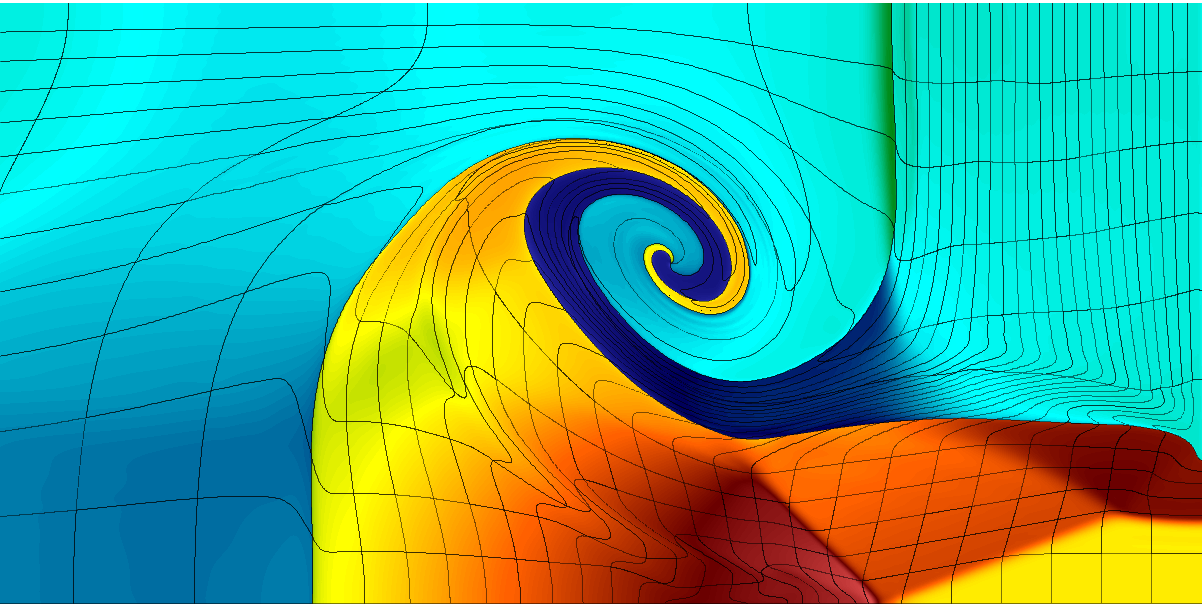
\includegraphics[scale = 0.15]{figs/triple-point_BLAST_q8q7.png} \\
            {\tiny Triple-Point problem with Q8-Q7}
          \end{tabular}
        \end{alertblock}
      \end{minipage}
    \end{center}
  \end{column}
  \begin{column}{0.30\textwidth}
    \begin{center}
      \begin{minipage}{0.95\textwidth}
        \begin{alertblock}{}
          \begin{center}
%          \begin{tabular}{c}
            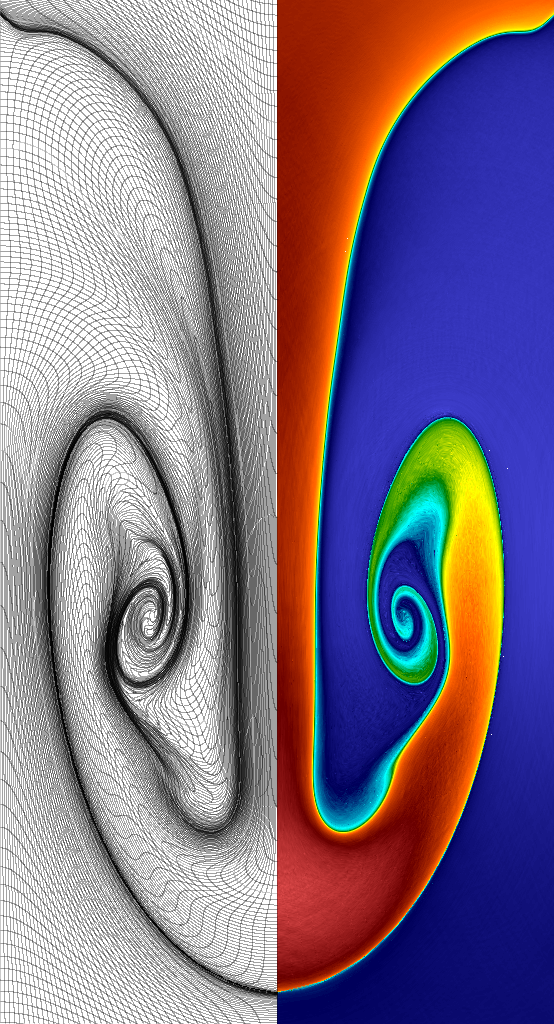
\includegraphics[scale = 0.1]{figs/q8q7_RT_density.png} \\
            {\tiny Rayleigh-Taylor Instability with Q8-Q7}
%          \end{tabular}
            \end{center}
      \end{alertblock}
    \end{minipage}
  \end{center}
\end{column}
\end{columns}

\begin{itemize}
\item \tiny{ https://computation.llnl.gov/casc/blast/blast.html}
\item \tiny{ Dobrev VA, Kolev TzV, Rieben RN. High order curvilinear finite element methods for Lagrangian hydrodynamics. SIAM J Sci Comput.}
\end{itemize}
\end{frame}


%===============================================================================
% NEW SLIDE
%===============================================================================
\begin{frame}\frametitle{Artificial Viscosity in BLAST}
\begin{block}{}
{\small``Our idea is to introduce (artificial) dissipative terms into the
equations so as to give the shocks a thickness comparable to (but preferably
somewhat larger than) the spacing of the points of the network... Then the
differential equations ...may be used for the entire calculation, just as
though there were no shocks at all.'' -- Von Neumann and Richtmyer}\\
\end{block}
\bigskip

Ideally, an artifical viscosity implementation should:
\begin{itemize}
  \item Always reduces kinetic energy (dissipates shocks)
  \item Vanishes in smooth regions and in rarefaction
  \item Vanishes in uniform contraction and rigid rotation
  \item Satisfies Rankine-Hugoniot jump conditions away from the shock
  \item Galilean invariant

\bigskip
\begin{block}{Artificial Stress in BLAST}
\[
\sigma_a = \mu\frac{1}{2}(\nabla v+v\nabla)\,,\quad\text{where}\quad
\mu\equiv\rho(q_2l_s^2|\Delta_sv|+q_1l_sc_s)\,.
\]
\end{block}
\item This allows us to robustly handle shocks, but limits our convergence to first order in smooth flow.
\end{itemize}
\end{frame}


%===============================================================================
% NEW SLIDE
%===============================================================================
\begin{frame}\frametitle{Sub-Cell Shock Capturing of Persson and Peraire}
% Mention idea comes from Persson
\begin{itemize}
\item Discontinuities create oscillations in the highest polynomial modes.
\item Persson and Peraire
\footnote{P. Persson, J. Peraire, Sub-Cell Shock Capturing for Discontinuous
Galerkin Methods, 44th AIAA Aerospace Sciences Meeting and Exhibit, Reno,
Nevada, 2007. AIAA-2007-513}
do a change of basis to a hierarchical family of orthogonal polynomials, such that
\[
u=\sum_{i=1}^{N(k)}u_{i}\psi_i\,,
\]
where $u$ is some function of the solution (velocity, entropy, etc).
\item Define a truncated expansion
\[
\tilde u=\sum_{i=1}^{N(k-1)}u_{i}\psi_i\,.
\]
\item Compute a piece-wise constant smoothness indicator using numerical quadrature,
\[
s_z=\log_{10}\frac{(u-\tilde u,u-\tilde u)_z}{(u,u)_z}\,.
\]
\item They then turn this into an artificial viscosity that vanishes for smooth, resolved flow.
\item In practice, this allows their high-order DG methods to achieve sub-zonal shock capturing.
\end{itemize}
\end{frame}


%===============================================================================
% NEW SLIDE
%===============================================================================
\begin{frame}\frametitle{Multi-Resolution Viscosity Limiter in BLAST}
\begin{itemize}
\item Persson and Peraire use discontinuous spaces, which makes the orthogonal basis expansion straight-forward.
\item In BLAST, it makes more sense to do an $L^2$ projection using our continuous velocity space.
\item For $v\in\mathcal{P}^k$, find $\mathbf{\tilde v}\in\mathcal{P}^{k-1}$ such that
\begin{align*}
\int_\Omega \mathbf{\tilde vw}dx&=\int_\Omega vwdx\quad\forall w\in\mathcal{P}^{p-1}\,.
\end{align*}
In matrix vector form, this is
\begin{align*}
\mathbf{M}_{k-1}\tilde v&=\mathbf{g_v}\,.
\end{align*}
\item Use the difference as a shock detector which we call the smoothness.
\[
s_z=\log_{10}||v-\tilde v||_z^2\,.
\]
\item Define a viscosity limiter.
\[
\psi_l=
\begin{cases}
0 &\text{if}\quad s_z <= s_0-\kappa\\
\frac{1}{2}\left(1+\sin\frac{\pi(s_z-s_0}{2\kappa}\right) &\text{if}\quad s_0-\kappa < s_z < s_0 + \kappa\\
1 &\text{if}\quad s_z >= s_0 + \kappa
\end{cases}
\]
where $s_0$ and $\kappa$ are tunable parameters that define the cutoff and transition region.
\item Use the new limited viscosity.
\[
\mu_l = \psi_l\mu
\]
\end{itemize}
\end{frame}


%===============================================================================
% NEW SLIDE
%===============================================================================
\begin{frame} \frametitle{High-order FEM overview: Time integration}
Let $Y = \left(\mathbf{v}; \mathbf{e}; \mathbf{x}\right)$. Then
the semi-discrete equations can be written in the form:
\vspace{-2.5mm}
\begin{columns}
\begin{column}{0.3\textwidth}
  \begin{center}
  \begin{minipage}{0.8\textwidth}
  \begin{block}{}
  \centering
  $\dfrac{\dd Y}{\dd t} = \mathcal{F}(Y, t)$
  \end{block}
  \end{minipage}
  \end{center}
\end{column}
\begin{column}{0.7\textwidth}
  \begin{center}
  \begin{minipage}{0.8\textwidth}
  \begin{alertblock}{}
  \centering
  $
    \mathcal{F}(Y, t) =
    \begin{pmatrix}
    \mathcal{F}_v(\mathbf{v}, \mathbf{e}, \mathbf{x}) \\
    \mathcal{F}_e(\mathbf{v}, \mathbf{e}, \mathbf{x}) \\
    \mathcal{F}_x(\mathbf{v}, \mathbf{e}, \mathbf{x})\\
    \end{pmatrix}
    =
    \begin{pmatrix}
    - \mathbf{M_v}^{\!\!-1} \mathbf{F}\cdot \mathbf{1} \\
    \mathbf{M_e}^{\!\!-1} \mathbf{F}^\top \cdot \mathbf{v} \\
    \mathbf{v}\\
    \end{pmatrix}
  $
  \end{alertblock}
  \end{minipage}
  \end{center}
\end{column}
\end{columns}
\medskip
Standard high-order time integration techniques (e.g.\ explicit Runge-Kutta
methods) can be applied to this system of nonlinear ODEs.

\medskip

The $L^2$ projection is done at each stage of the integration and used in the artificial viscosity when computing $\mathbf{F}$.

\medskip

For example, consider the \myem{energy conserving} RK2Avg method:
\begin{center}
\begin{minipage}[c]{0.425\textwidth}\begin{alertblock}{}\centering
$
\begin{aligned}
\mathbf{\tilde v} &= \mathbf{M}_{k-1}^{-1}\mathbf{g_v}\\
\mathbf{v}^{n+\frac{1}{2}} &= \mathbf{v}^{n} - (\Delta t/2)\, \mathbf{M_v}^{\!\!-1} \mathbf{F}^n\cdot \mathbf{1} \\
\mathbf{e}^{n+\frac{1}{2}} &= \mathbf{e}^{n} + (\Delta t/2)\, \mathbf{M_e}^{\!\!-1} (\mathbf{F}^n)^\top \cdot \mathbf{v}^{n+\frac{1}{2}} \\
\mathbf{x}^{n+\frac{1}{2}} &= \mathbf{x}^{n} + (\Delta t/2)\, \mathbf{v}^{n+\frac{1}{2}}\\
\end{aligned}
$
\end{alertblock}\end{minipage}
\hspace{0.09\textwidth}
\begin{minipage}[c]{0.425\textwidth}\begin{alertblock}{}\centering
$
\begin{aligned}
\mathbf{\tilde v} &= \mathbf{M}_{k-1}^{-1}\mathbf{g_v}\\
\mathbf{v}^{n+1} &= \mathbf{v}^{n} - \Delta t\,  \mathbf{M_v}^{\!\!-1} \mathbf{F}^{n+\frac{1}{2}}\cdot \mathbf{1} \\
\mathbf{e}^{n+1} &= \mathbf{e}^{n} + \Delta t\,  \mathbf{M_e}^{\!\!-1} (\mathbf{F}^{n+\frac{1}{2}})^\top \cdot \bar{\mathbf{v}}^{n+\frac{1}{2}} \\
\mathbf{x}^{n+1} &= \mathbf{x}^{n} +  \Delta t\, \bar{\mathbf{v}}^{n+\frac{1}{2}}\\
\end{aligned}
$
\end{alertblock}\end{minipage}
\end{center}

\end{frame}


%===============================================================================
% NEW SLIDE
%===============================================================================
\begin{frame}\frametitle{Taylor Green Vortex, $s_0=-11$, $\kappa=1$}
\begin{itemize}
\item On coarse meshes, the indicator does not detect sufficient smoothness
in the solution to turn off viscosity.
\item With sufficient resolution, the indicator shuts down all viscosity and we
recover higher order convergence rates.
\end{itemize}
\begin{columns}
\begin{column}{0.25\textwidth}
\centering{Q2-Q1}
\vspace{-4ex}
\begin{figure}[t]
\begin{center}
\includegraphics<1>[height=0.8\textwidth]{figs/TG-2/Q2-smoothness-4.png}
\includegraphics<2>[height=0.8\textwidth]{figs/TG-2/Q2-smoothness-5.png}
\includegraphics<3>[height=0.8\textwidth]{figs/TG-2/Q2-smoothness-6.png}
\includegraphics<4>[height=0.8\textwidth]{figs/TG-2/Q2-smoothness-7.png}
\small{\\Smoothness}
\end{center}
\end{figure}
\begin{figure}[t]
\begin{center}
\includegraphics<1>[height=0.8\textwidth]{figs/TG-2/Q2-limiter-4.png}
\includegraphics<2>[height=0.8\textwidth]{figs/TG-2/Q2-limiter-5.png}
\includegraphics<3>[height=0.8\textwidth]{figs/TG-2/Q2-limiter-6.png}
\includegraphics<4>[height=0.8\textwidth]{figs/TG-2/Q2-limiter-7.png}
\small{\\Limiter}
\end{center}
\end{figure}
\end{column}
\begin{column}{0.25\textwidth}
\centering{Q4-Q3}
\vspace{-4ex}
\begin{figure}[t]
\begin{center}
\includegraphics<1>[height=0.8\textwidth]{figs/TG-2/Q4-smoothness-4.png}
\includegraphics<2>[height=0.8\textwidth]{figs/TG-2/Q4-smoothness-5.png}
\includegraphics<3>[height=0.8\textwidth]{figs/TG-2/Q4-smoothness-6.png}
\includegraphics<4>[height=0.8\textwidth]{figs/TG-2/Q4-smoothness-7.png}
\small{\\Smoothness}
\end{center}
\end{figure}
\begin{figure}[t]
\begin{center}
\includegraphics<1>[height=0.8\textwidth]{figs/TG-2/Q4-limiter-4.png}
\includegraphics<2>[height=0.8\textwidth]{figs/TG-2/Q4-limiter-5.png}
\includegraphics<3>[height=0.8\textwidth]{figs/TG-2/Q4-limiter-6.png}
\includegraphics<4>[height=0.8\textwidth]{figs/TG-2/Q4-limiter-7.png}
\small{\\Limiter}
\end{center}
\end{figure}
\end{column}
\begin{column}{0.5\textwidth}
\begin{figure}[t]
\begin{center}
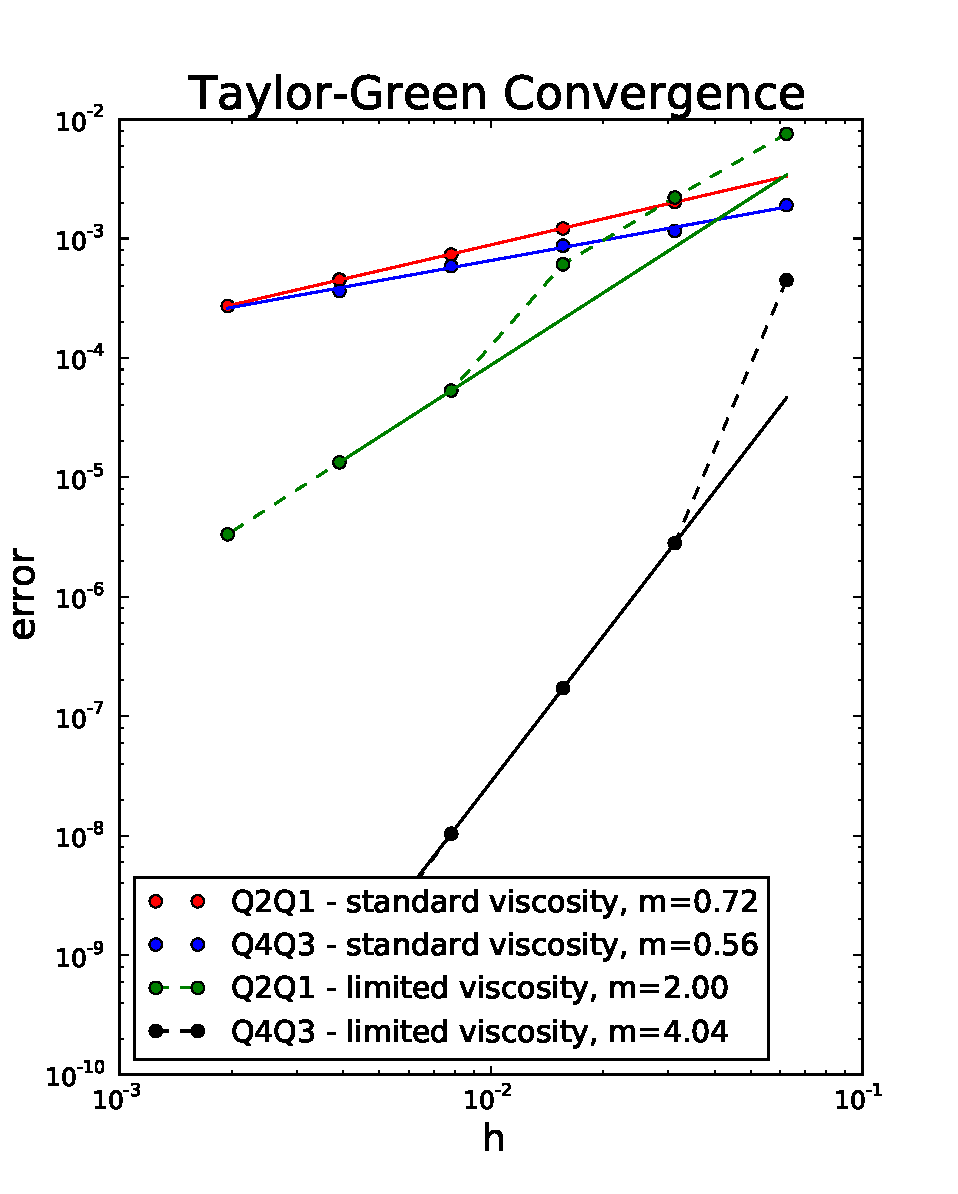
\includegraphics[width=0.8\textwidth]{figs/TGConvergence.pdf}
\end{center}
\end{figure}
\end{column}
\end{columns}
\end{frame}


%===============================================================================
% NEW SLIDE
%===============================================================================
\begin{frame}\frametitle{Sod Shock Tube, $s_0=9.5$, $\kappa=0.5$}
\vspace{-1ex}
Q4-Q3 elements on a 50x1 mesh
\vspace{-2ex}
\begin{columns}
\begin{column}{0.3\textwidth}
\begin{figure}[t]
\begin{center}
Smoothness
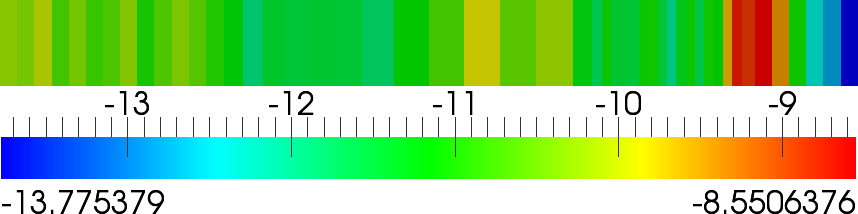
\includegraphics[width=1.0\textwidth]{figs/Sod/Q4l-50-smoothness.png}
\end{center}
\end{figure}
\begin{figure}[t]
\begin{center}
Limiter
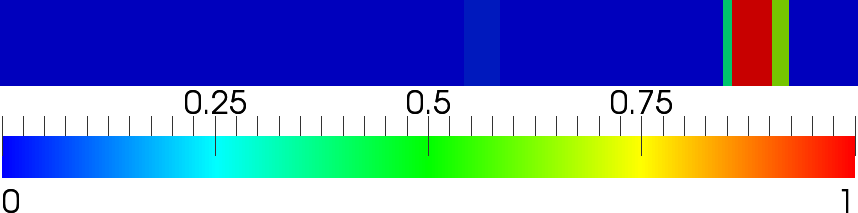
\includegraphics[width=1.0\textwidth]{figs/Sod/Q4l-50-limiter.png}
\end{center}
\end{figure}
\begin{figure}[t]
\begin{center}
Viscosity with Limiter
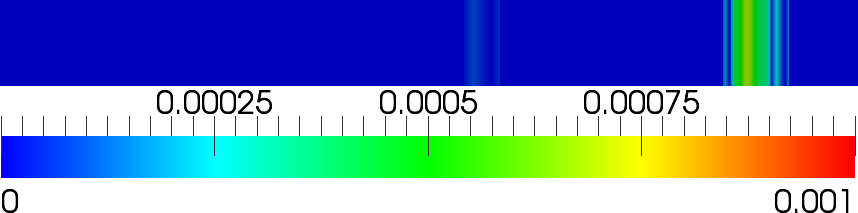
\includegraphics[width=1.0\textwidth]{figs/Sod/Q4l-50-viscosity.png}
\end{center}
\end{figure}
\begin{figure}[t]
\begin{center}
Viscosity without Limiter
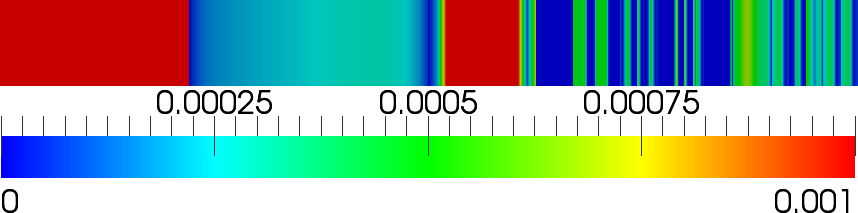
\includegraphics[width=1.0\textwidth]{figs/Sod/Q4nl-50-viscosity.png}
\end{center}
\end{figure}
\end{column}
\begin{column}{0.7\textwidth}
\begin{center}
Density\\
\includegraphics<1>[width=0.8\textwidth]{figs/Sod/Q4-50-Density.png}
\includegraphics<2>[width=0.8\textwidth]{figs/Sod/Q4-50-Density-zoom.png}
\end{center}
\end{column}
\end{columns}
\end{frame}


%===============================================================================
% NEW SLIDE
%===============================================================================
\begin{frame}\frametitle{Sedov Blast Wave, $s_0=-9.5$, $\kappa=0.5$}
\vspace{1ex}
Q4-Q3 elements on an 80x80 mesh
\vspace{-4ex}
\begin{columns}
\begin{column}{0.3\textwidth}
\begin{figure}[t]
\begin{center}
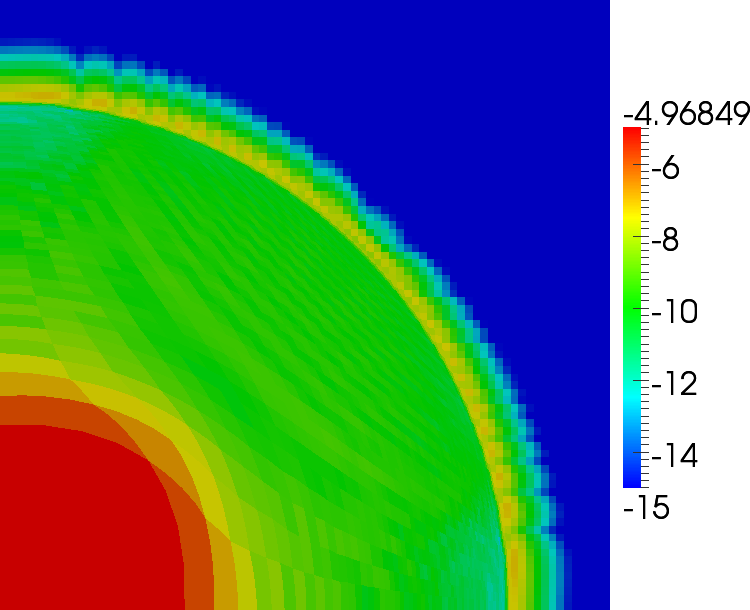
\includegraphics[height=0.9\textwidth]{figs/Sedov/Q2l-80-smoothness.png}
\\Smoothness
\end{center}
\end{figure}
\begin{figure}[t]
\begin{center}
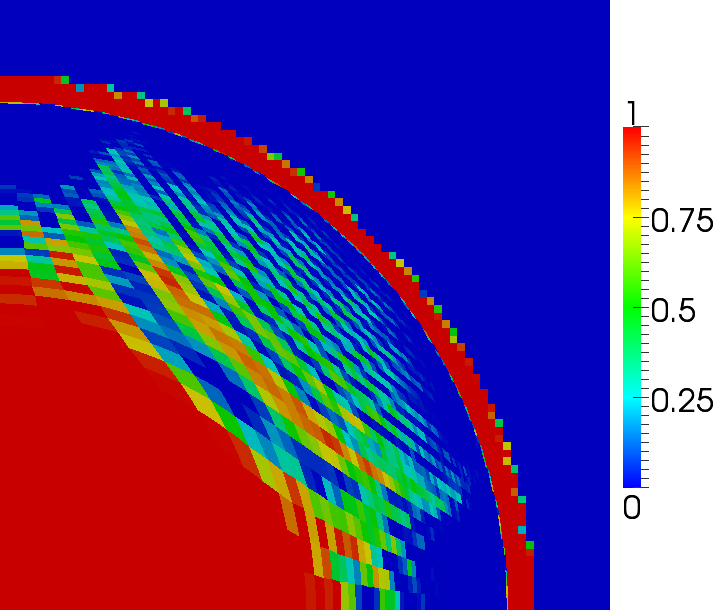
\includegraphics[height=0.9\textwidth]{figs/Sedov/Q2l-80-limiter.png}
\\Limiter
\end{center}
\end{figure}
\end{column}
\begin{column}{0.3\textwidth}
\begin{figure}[t]
\begin{center}
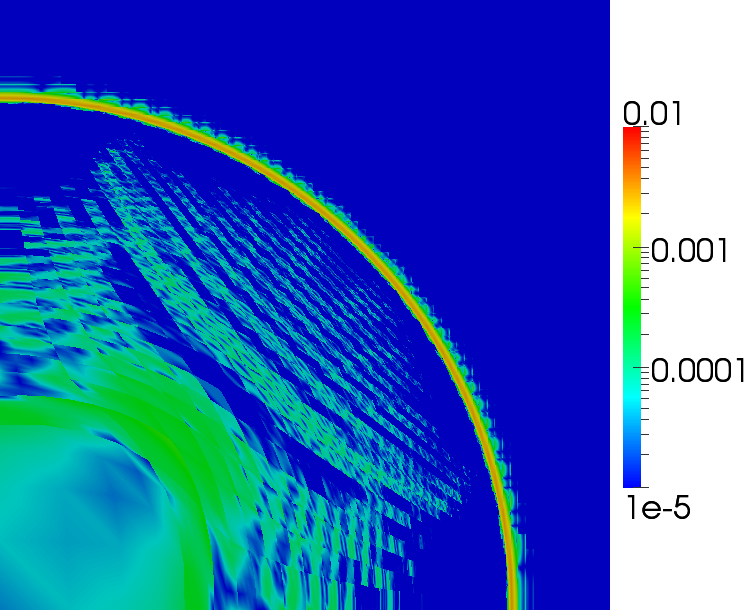
\includegraphics[height=0.9\textwidth]{figs/Sedov/Q2l-80-viscosity.png}
\\Viscosity with Limiter
\end{center}
\end{figure}
\begin{figure}[t]
\begin{center}
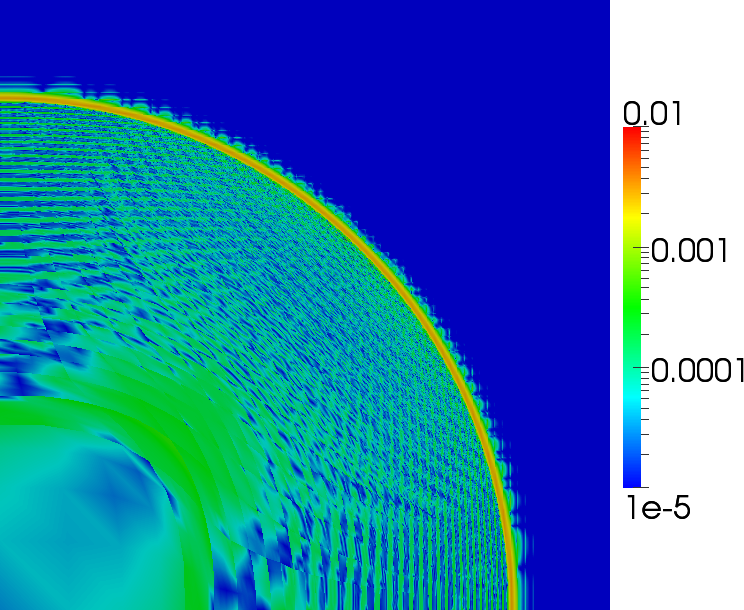
\includegraphics[height=0.9\textwidth]{figs/Sedov/Q2nl-80-viscosity.png}
\\Viscosity without Limiter
\end{center}
\end{figure}
\end{column}
\begin{column}{0.3\textwidth}
\begin{figure}[t]
\begin{center}
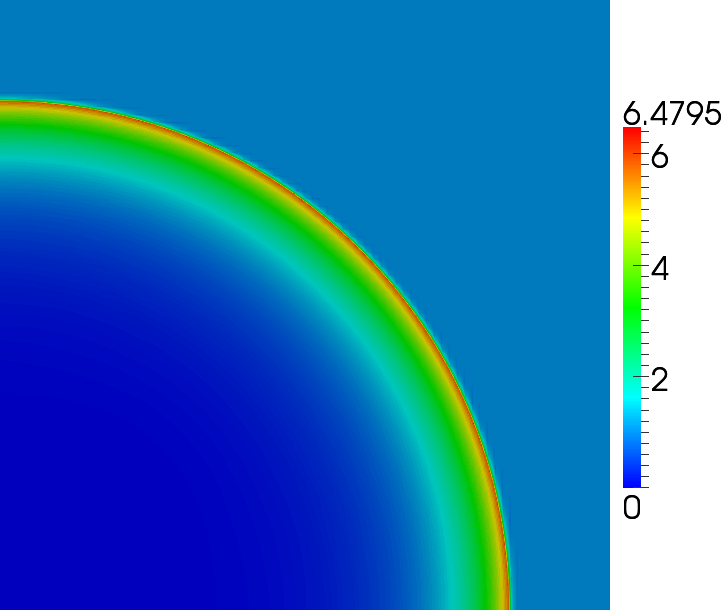
\includegraphics[height=0.9\textwidth]{figs/Sedov/Q2l-80-density.png}
\\Density with Limiter
\end{center}
\end{figure}
\begin{figure}[t]
\begin{center}
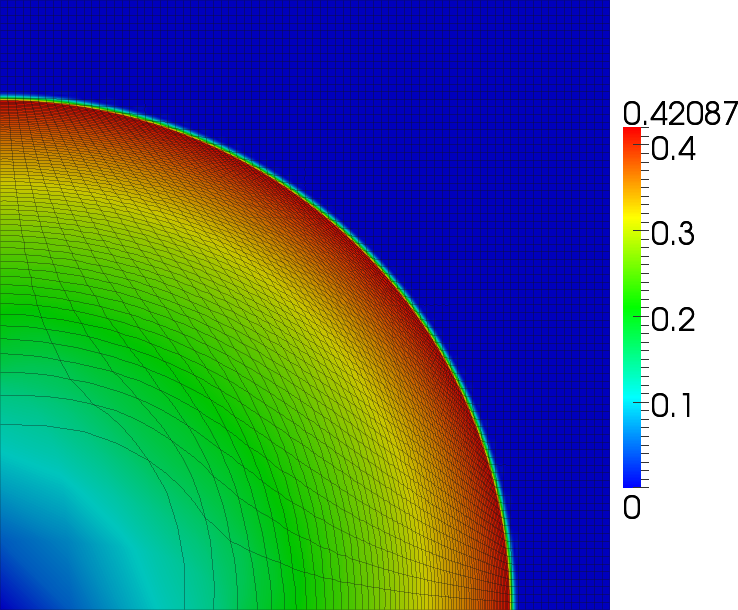
\includegraphics[height=0.9\textwidth]{figs/Sedov/Q2l-80-velocity.png}
\\Velocity with Limiter
\end{center}
\end{figure}
\end{column}
\end{columns}
\end{frame}


%===============================================================================
% NEW SLIDE
%===============================================================================
\begin{frame}\frametitle{Noh Implosion, $s_0=-9.5$, $\kappa=0.5$}
\vspace{1ex}
Q2-Q1 elements on an 128x128 mesh
\vspace{-4ex}
\begin{columns}
\begin{column}{0.3\textwidth}
\begin{figure}[t]
\begin{center}
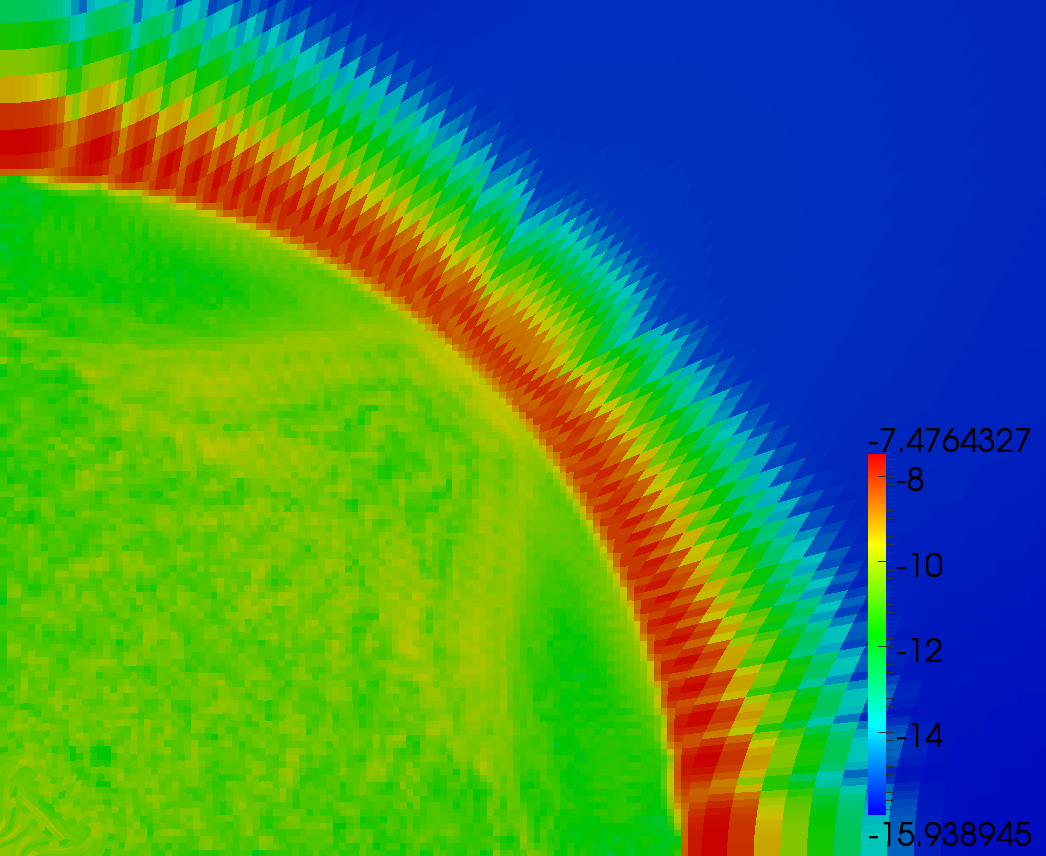
\includegraphics[height=0.9\textwidth]{figs/Noh/Q2l-7-smoothness.png}
\\Smoothness
\end{center}
\end{figure}
\begin{figure}[t]
\begin{center}
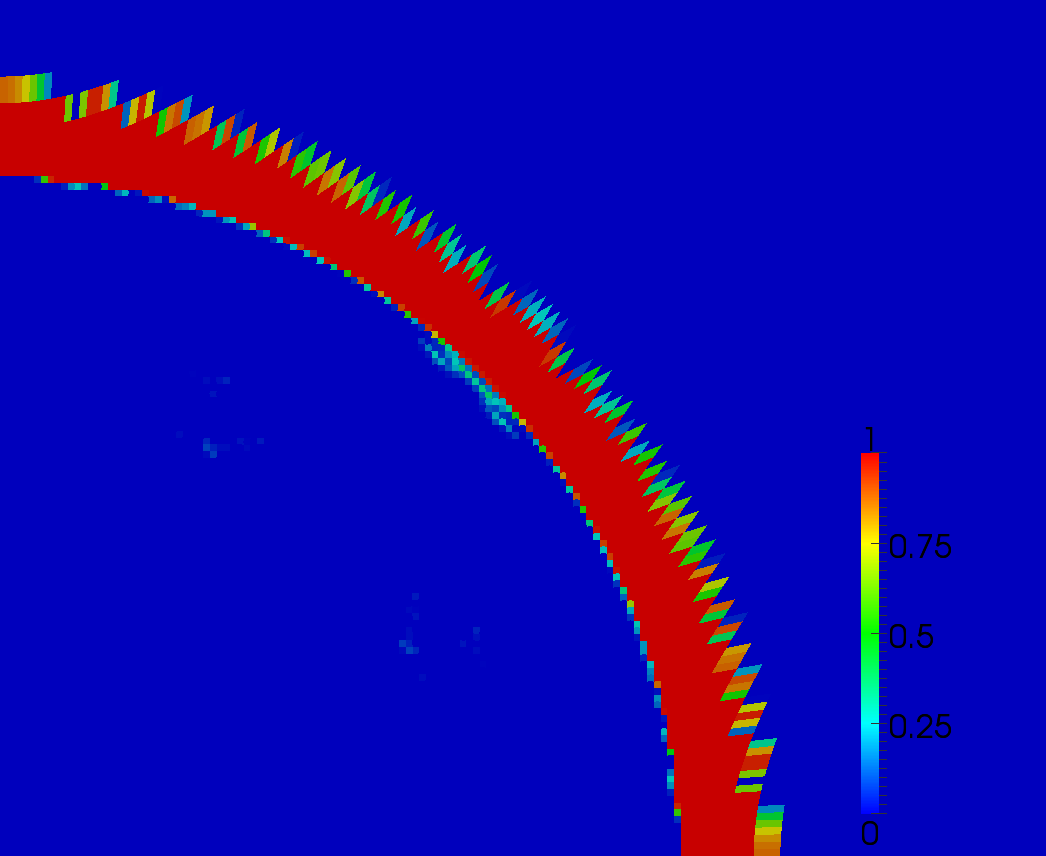
\includegraphics[height=0.9\textwidth]{figs/Noh/Q2l-7-limiter.png}
\\Limiter
\end{center}
\end{figure}
\end{column}
\begin{column}{0.3\textwidth}
\begin{figure}[t]
\begin{center}
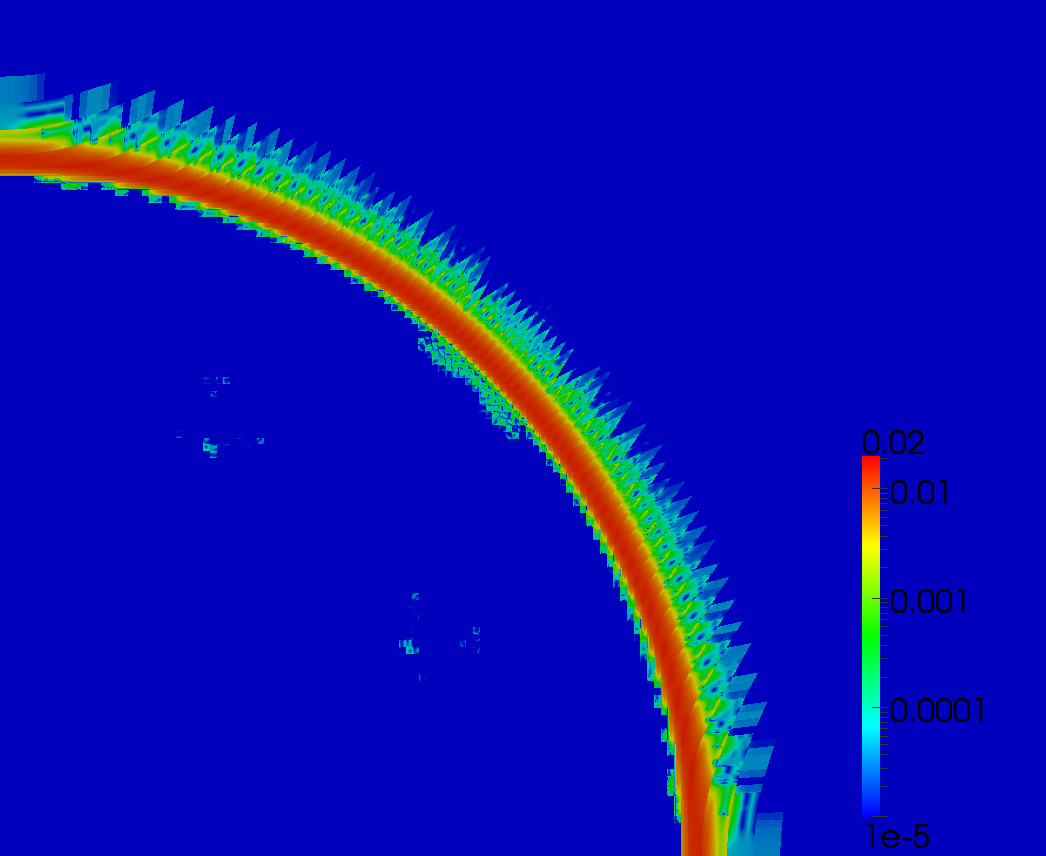
\includegraphics[height=0.9\textwidth]{figs/Noh/Q2l-7-viscosity.png}
\\Viscosity with Limiter
\end{center}
\end{figure}
\begin{figure}[t]
\begin{center}
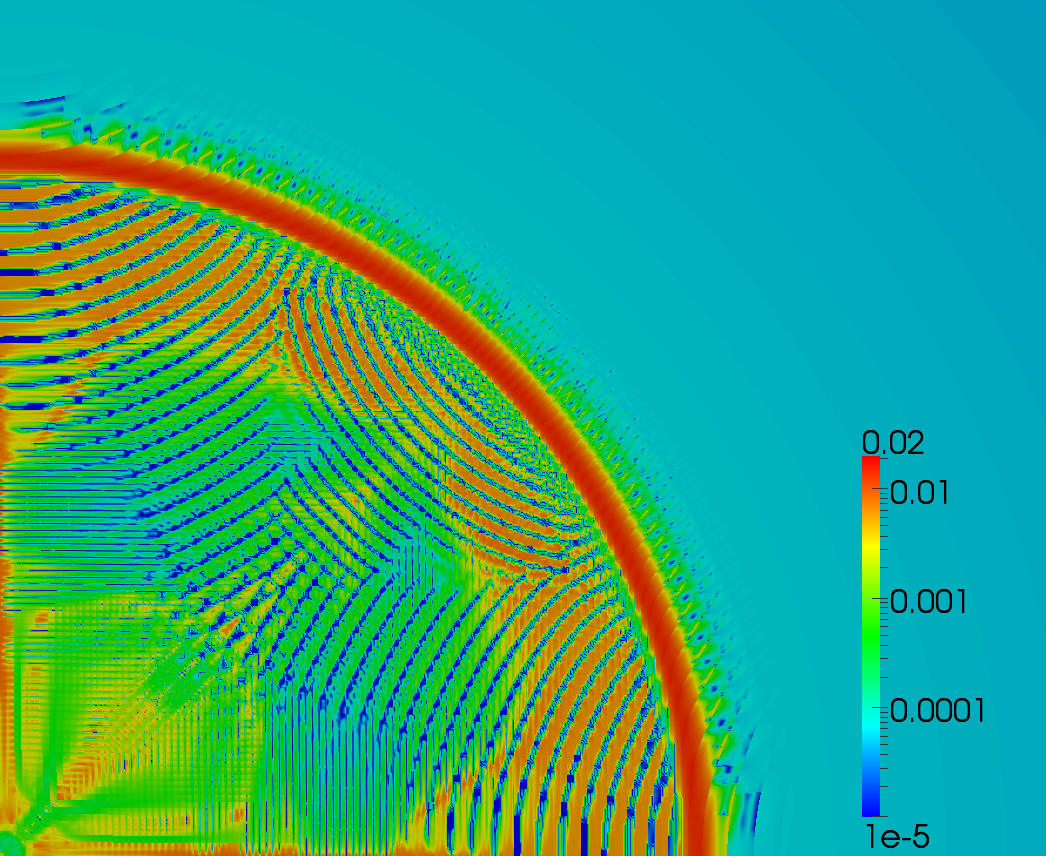
\includegraphics[height=0.9\textwidth]{figs/Noh/Q2nl-7-viscosity.png}
\\Viscosity without Limiter
\end{center}
\end{figure}
\end{column}
\begin{column}{0.3\textwidth}
\begin{figure}[t]
\begin{center}
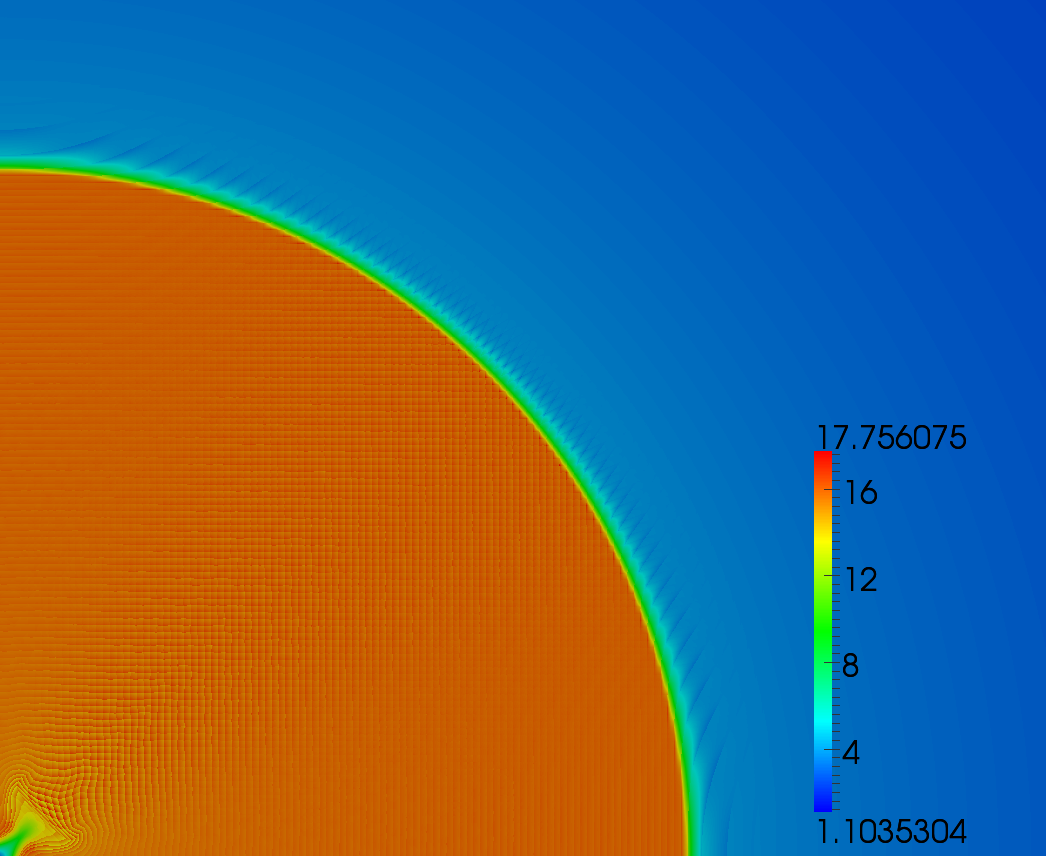
\includegraphics[height=0.9\textwidth]{figs/Noh/Q2l-7-density.png}
\\Density with Limiter
\end{center}
\end{figure}
\begin{figure}[t]
\begin{center}
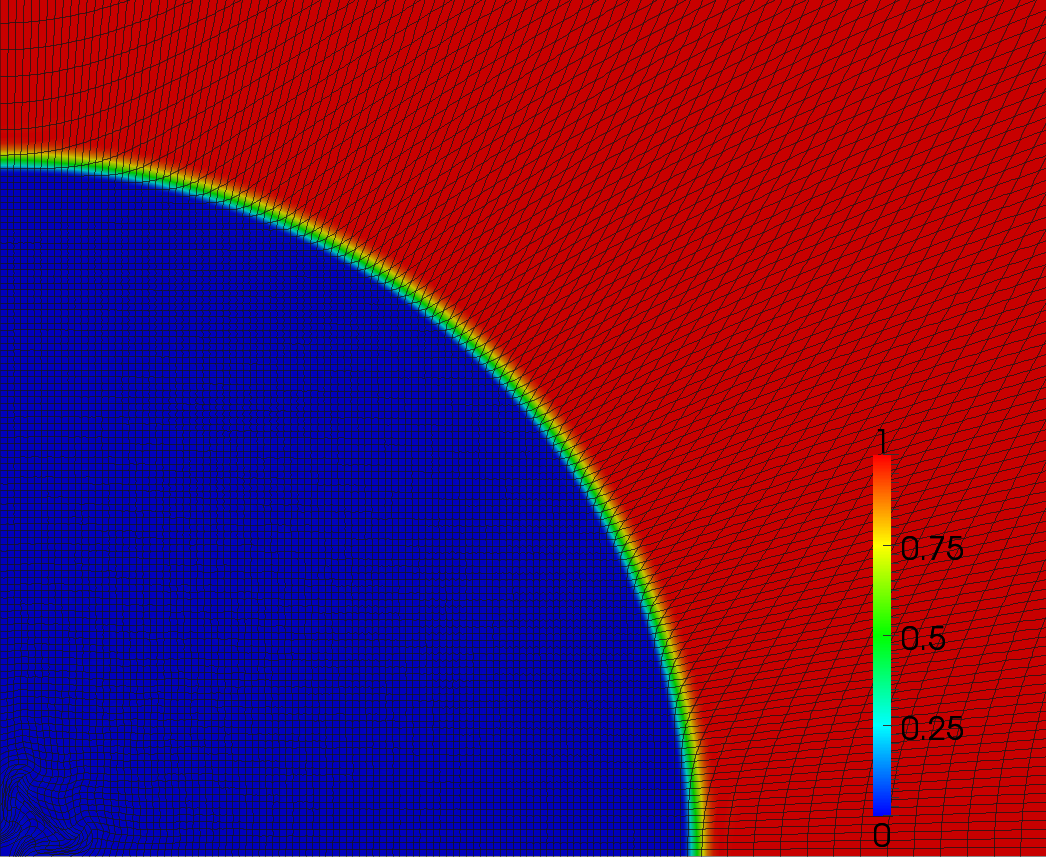
\includegraphics[height=0.9\textwidth]{figs/Noh/Q2l-7-velocity.png}
\\Velocity with Limiter
\end{center}
\end{figure}
\end{column}
\end{columns}
\end{frame}


%===============================================================================
% NEW SLIDE
%===============================================================================
\begin{frame}\frametitle{Noh Implosion, $s_0=-9.5$, $\kappa=0.5$}
\begin{columns}
\begin{column}{0.35\textwidth}
\begin{center}
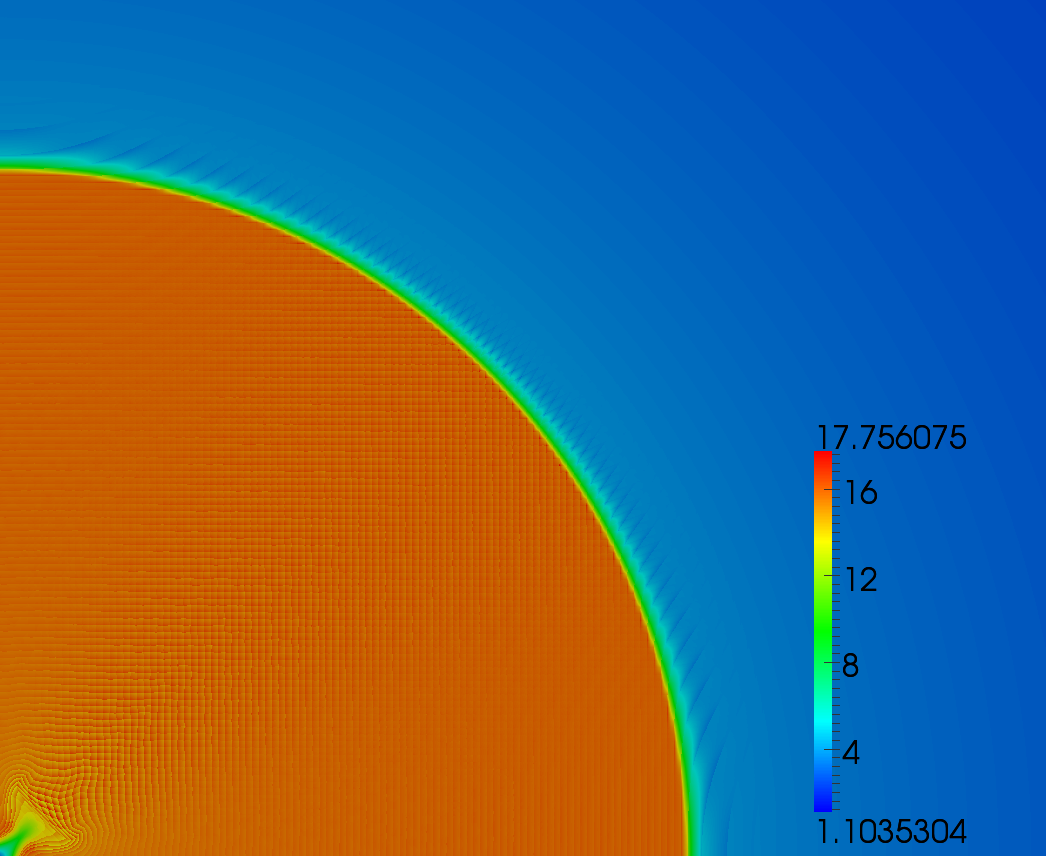
\includegraphics[height=0.9\textwidth]{figs/Noh/Q2l-7-density.png}
\\Density with Limiter
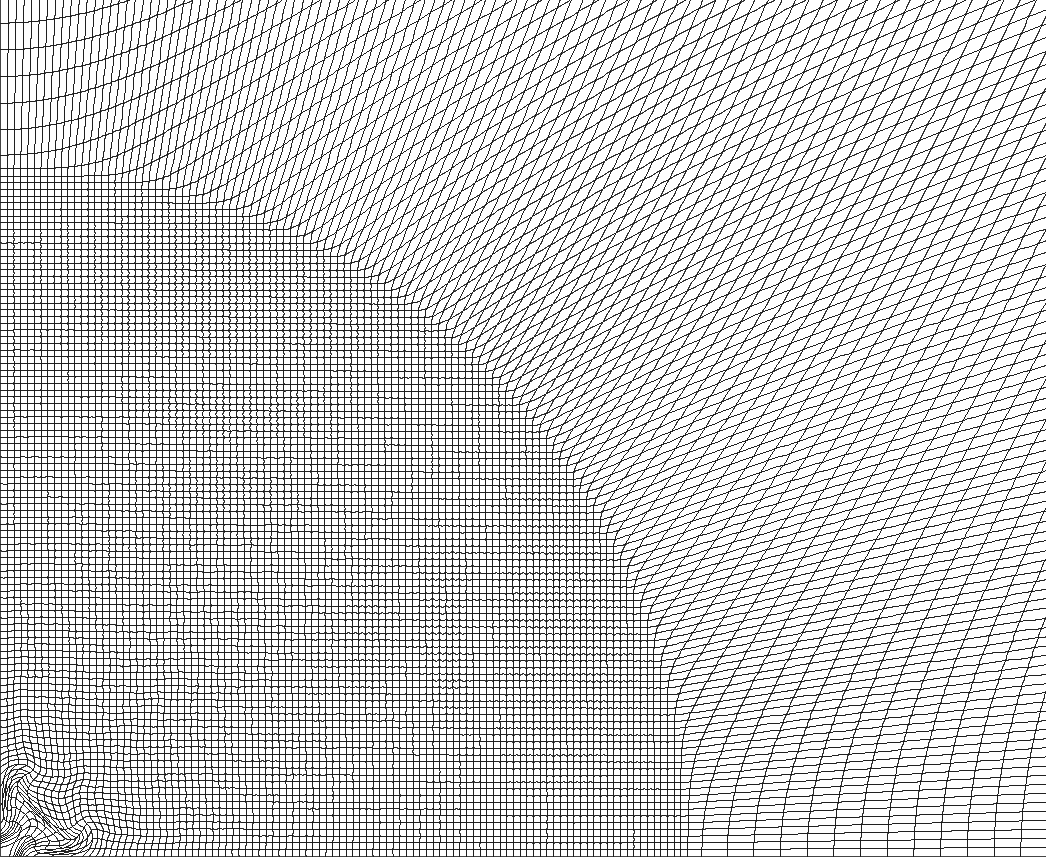
\includegraphics[height=0.9\textwidth]{figs/Noh/Q2l-7-mesh.png}
\\Mesh with Limiter
\end{center}
\end{column}
\begin{column}{0.35\textwidth}
\begin{center}
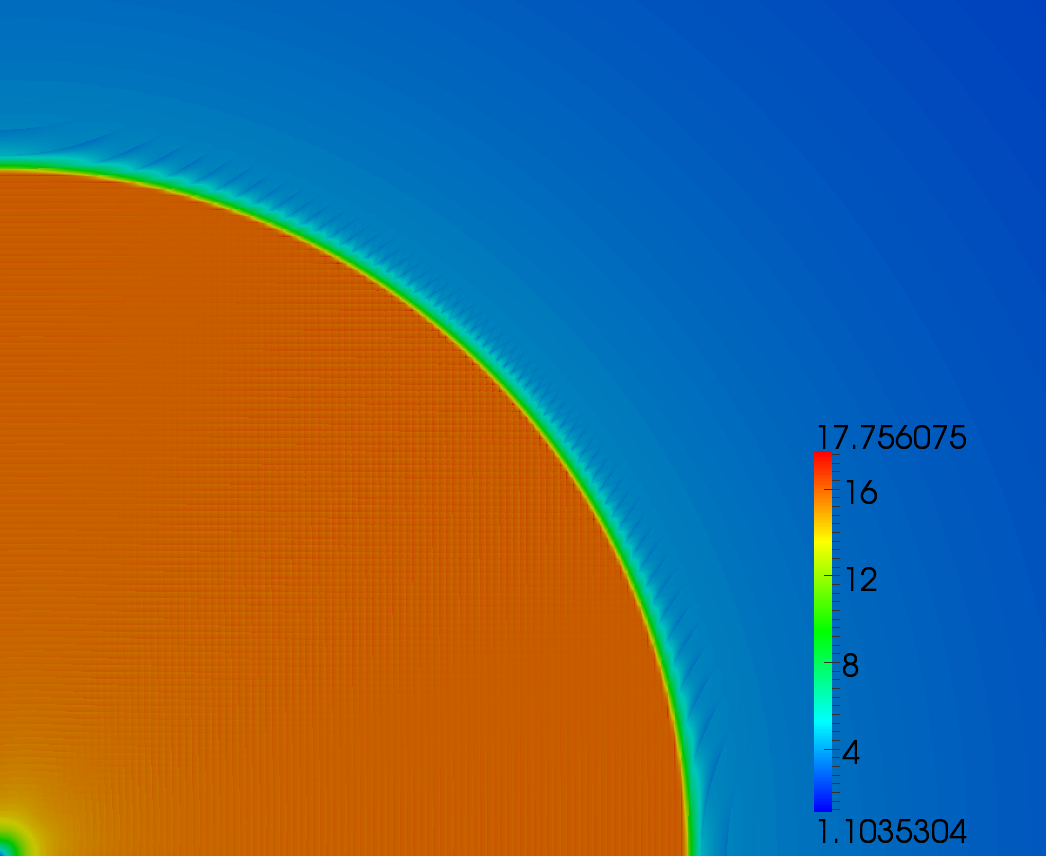
\includegraphics[height=0.9\textwidth]{figs/Noh/Q2nl-7-density.png}
\\Density without Limiter
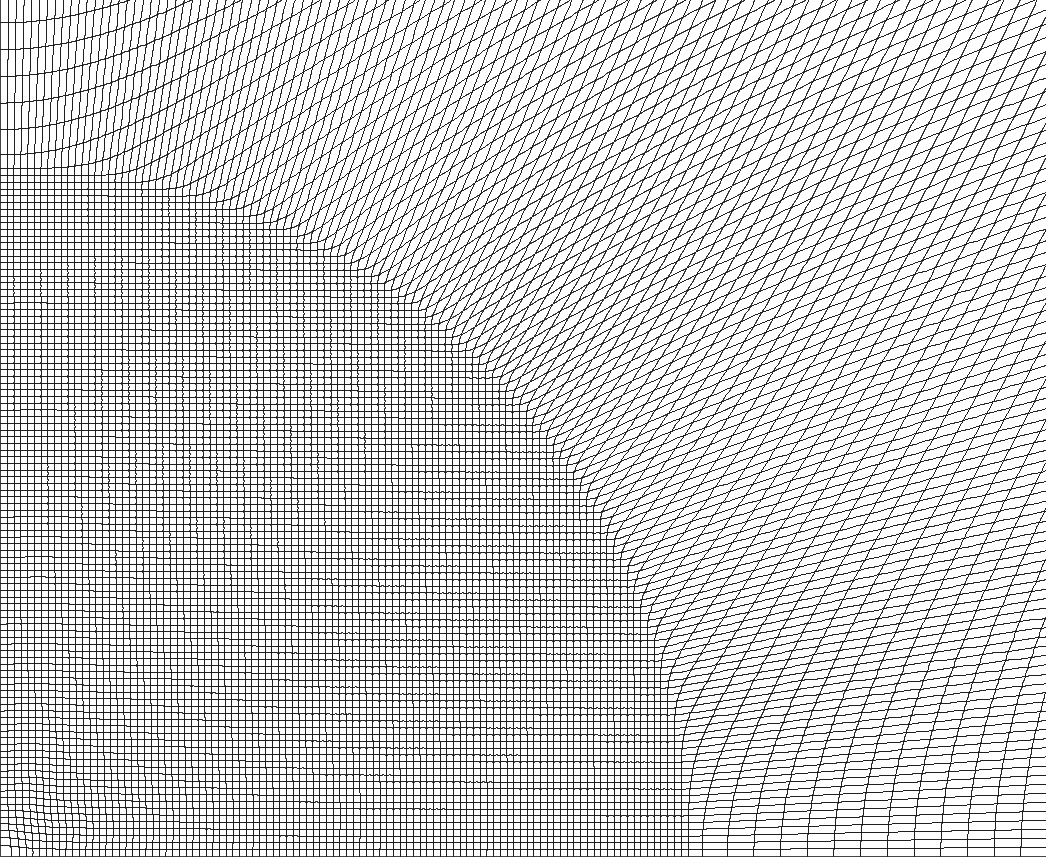
\includegraphics[height=0.9\textwidth]{figs/Noh/Q2nl-7-mesh.png}
\\Mesh without Limiter
\end{center}
\end{column}
\end{columns}
\end{frame}


%===============================================================================
% NEW SLIDE
%===============================================================================
\begin{frame}\frametitle{Triple Point Shockwave, $s_0=-9.5$, $\kappa=0.5$}
\vspace{1ex}
% Q2-Q1 elements
\vspace{-4ex}
\small{
\begin{columns}
\begin{column}{0.45\textwidth}
\begin{center}
Smoothness\\
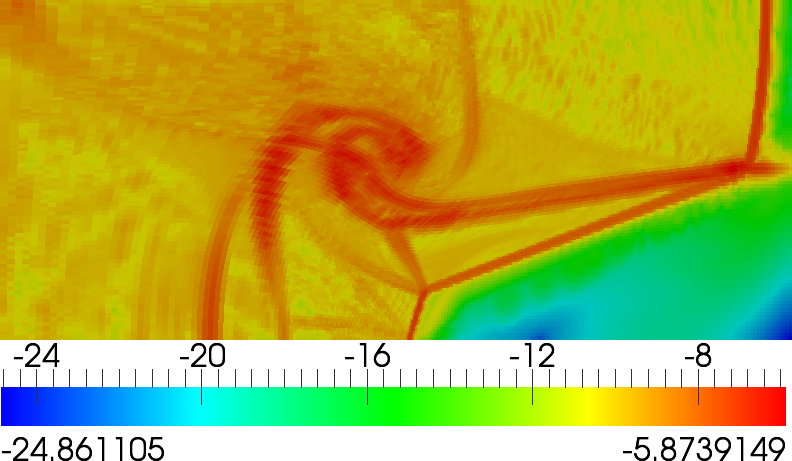
\includegraphics[width=0.8\textwidth]{figs/TriplePt/Q2-4-smoothness-limiter.png}\\
Viscosity with Limiter\\
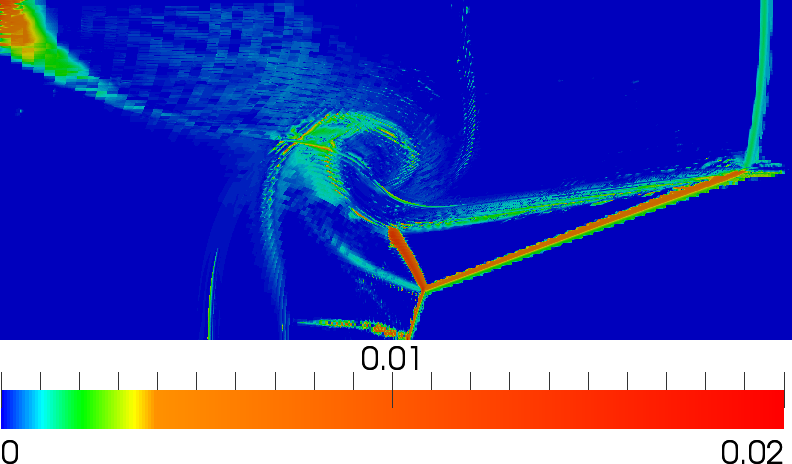
\includegraphics[width=0.8\textwidth]{figs/TriplePt/Q2-4-viscosity-limiter.png}\\
Density with Limiter\\
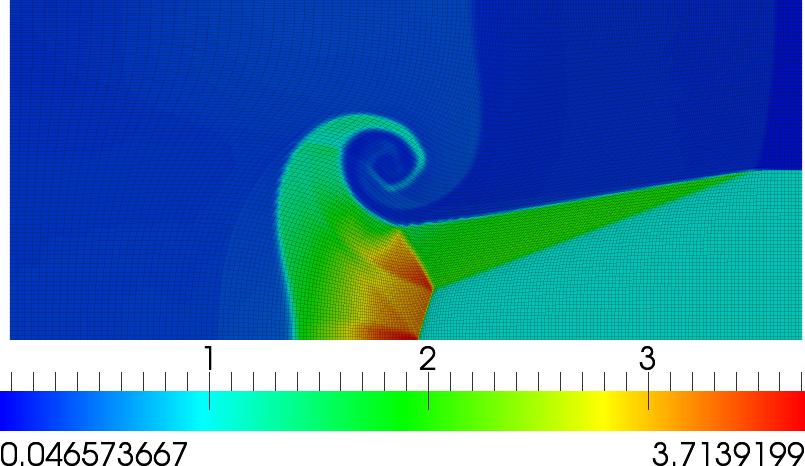
\includegraphics[width=0.8\textwidth]{figs/TriplePt/Q2-4-density-limiter.png}\\
\end{center}
\end{column}
\begin{column}{0.45\textwidth}
\begin{center}
Limiter\\
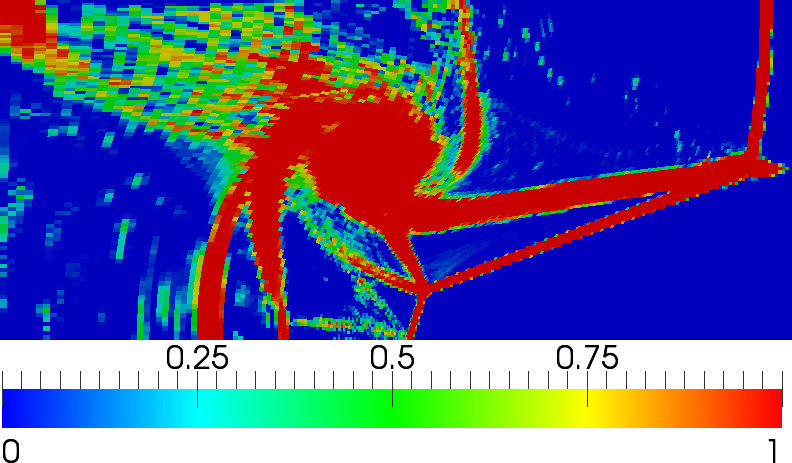
\includegraphics[width=0.8\textwidth]{figs/TriplePt/Q2-4-limiter-limiter.png}\\
Viscosity without Limiter\\
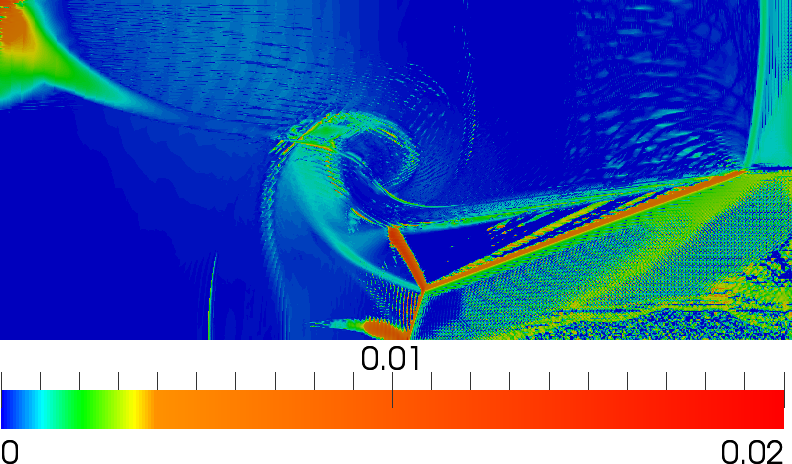
\includegraphics[width=0.8\textwidth]{figs/TriplePt/Q2-4-viscosity-nolimiter.png}\\
Density without Limiter\\
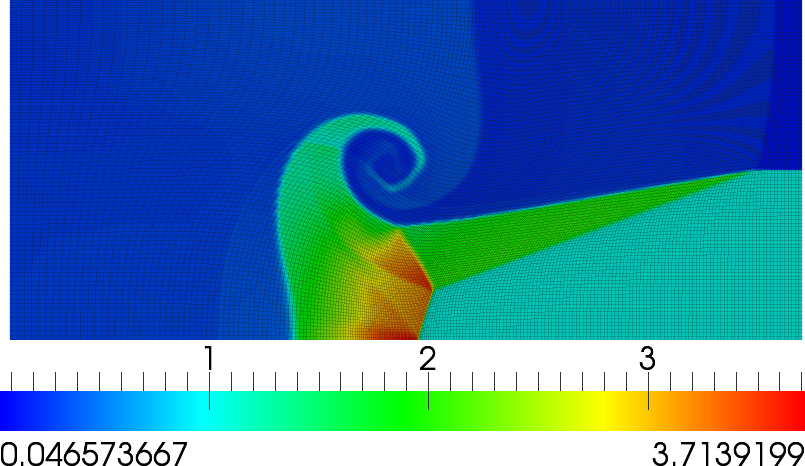
\includegraphics[width=0.8\textwidth]{figs/TriplePt/Q2-4-density-nolimiter.png}\\
\end{center}
\end{column}
\end{columns}
}
\end{frame}


%===============================================================================
% NEW SLIDE
%===============================================================================
\begin{frame}\frametitle{Conclusions}
\begin{block}{Future work}
\begin{itemize}
\item Try using physical mass matrices in $L^2$ projection.
\begin{itemize}
\item Don't need to recompute at each time step.
\end{itemize}
\item Try expanding velocity in terms of orthonormal Legendre polynomials as per Persson and Peraire.
\item Consider making $s_0$ and $kappa$ functions of $h$ and/or $p$.
\end{itemize}
\end{block}
\end{frame}


% \bibliographystyle{plain}
% {\scriptsize
% \bibliography{../DPG.bib}
% }

\end{document}
